\documentclass[12pt,fleqn]{article}

\newcommand{\mbm}[1]{\mbox{\boldmath $#1$}}
\newcommand{\norm}[1]{\lVert#1\rVert}


\usepackage[small,hang]{caption2}
\usepackage{graphicx}
\usepackage{bbold}
\usepackage{amsmath}
\usepackage{amssymb}
\usepackage{hyperref}
\usepackage{pdfpages}
\usepackage[          % set page and margin sizes
  a4paper,
  top=7mm,
  bottom=7mm,
  inner=20mm,
  outer=20mm,
  bindingoffset=0mm,
  head=10mm,
  foot=10mm,
  headsep=15mm,
  footskip=15mm,
  includeheadfoot,
]{geometry}
\usepackage{fancyhdr}
\pagestyle{fancy}
\fancyhead{}
\fancyfoot{}
\fancyhead[LO,LE]{Project Work}
\fancyhead[CO,CE]{--- Quadcopter Stabilization and Tracking ---}
\fancyhead[RO,RE]{May $27$, $2016$}
\fancyfoot[RO, LE] {\thepage}


%%%%%%%%%%%%%
%%Titlepage%%
%%%%%%%%%%%%%%

\begin{document}
\thispagestyle{empty}
\noindent\makebox[\linewidth]{\rule{.75\paperwidth}{0.4pt}}
\begin{center}
{\Large \textbf{{\"O}rebro University}}
\end{center}
\vspace{-4mm}
\noindent\makebox[\linewidth]{\rule{.75\paperwidth}{0.4pt}} \\
\vspace{4cm}
\begin{center}
{\Large\sffamily\bfseries
Project Work: \\[1ex]
Quadcopter Stabilization and Tracking \\[2ex]
}

\vspace{6cm}
\noindent\makebox[\linewidth]{\rule{.75\paperwidth}{0.4pt}}
{\large
\renewcommand{\arraystretch}{1.5}
  \begin{tabular}{l}
   \textbf{Anders Wikstr\"{o}m}\\
   (anders.wikstrom.88@gmail.com)\\
   \textbf{Chittaranjan Srinivas Swaminathan}\\
   (chitt@live.in)\\
 \end{tabular}}
\end{center}
\vspace{-2mm}
\noindent\makebox[\linewidth]{\rule{.75\paperwidth}{0.4pt}}
\newpage

\tableofcontents

\newpage


%%%%%%%%%%%%%%%%%%%%%%%%%
%%Beginning of document%%
%%%%%%%%%%%%%%%%%%%%%%%%%

\section*{Abstract}
Quadcopters are non-holonomic and non-linear systems that are highly
difficult to control. The aim of this project is to understand the
model and design a inverse dynamics controller for altitude stability
and trajectory tracking. In this report we present an Inverse Dynamics
controller, using which the quadcoptor is able to track trajectories
with an error magnitude less than $10^{-3}$. 

\section{Introduction}

\section{Dynamics}
In this section we describe the model of the quadcopter used in the
simulation and control. The following subsections detail the different
components of the dynamics.

\subsection{Forces and Torques}

In the following sections, the different forces and torques used in
the model are explained. In most cases, a simplified formula is used
for convenience. 

\subsubsection{Forces generated by the propellers}

The thrust from each propeller is proportional to the square of the
angular velocity of the motor \cite{Andrew}. Thus, the thrust from the
$i^{th}$ propeller could be written as:

$$ T_i = k\omega_i^2 $$

The thrust vector in the z-axis of the body frame, $\mbm{T_{B}}$, can
be written as, 

\begin{equation} \label{thrust}
$$ \mbm{T_{B}} = k \begin{bmatrix}0 \\ 0\\ \sum \limits_{i=1}^{4}
  \omega_i^2 \end{bmatrix} $$
\end{equation}

\subsubsection{Drag force on the quadcopter}
We model the drag force as a force proportional to the linear velocity
in each direction. 

$$ \mbm{F_D} = \begin{bmatrix} -k_d\dot{x}\\ -k_d\dot{y}\\
  -k_d\dot{z} \end{bmatrix} $$

Which can be written as 
\begin{equation} \label{dragforce}
$$ \mbm{F_D}= -k_d\mbm{\dot{x}}$$.
\end{equation}

\subsubsection{Torques generated by the propellers}

Again from \cite{Andrew}, the torque due to individual motors is also
proportional to the square of the angular velocity.

\begin{figure}
\centering
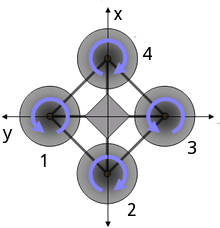
\includegraphics[scale=0.8]{quadrotor.png}
\caption{Quadrotor axes and rotor directions}
\label{quadrotor}
\end{figure}

$$ \tau = b\ \omega^2 $$

So the net torque in the z-axis of the body frame is,

\begin{equation} \label{taupsi}
$$ \tau_\psi = b\ (\omega_1^2 - \omega_2^2 + \omega_3^2 -
\omega_4^2) $$
\end{equation}

The roll and pitch torques are simply due the difference in torques
generated due to the thrust in the opposing motors. Let $L$ be the
length of each arm of the quadcoptor and, if motors 1 and 3 are along
the y-axis and motors 2 and 4 were along the x-axis (see fig. \ref{quadrotor}), the torque along
the x-axis is given by,

\begin{equation} \label{tauphi}
$$ \tau_\phi = L (k\omega_1^2 - k\omega_3^2) $$
\end{equation}

The torque along the y-axis is given by,
\begin{equation} \label{tautheta}
$$ \tau_\theta = L (k\omega_2^2 - k\omega_4^2) $$
\end{equation}

Putting the three components from \ref{taupsi}, \ref{tauphi} and
\ref{tautheta} together, we have the torque vector in the body frame as,

\begin{equation} \label{tauvector} 
$$ \mbm{\tau_B} = \begin{bmatrix} L (k\omega_1^2 - k\omega_3^2)\\ L
  (k\omega_2^2 - k\omega_4^2) \\ b\ (\omega_1^2 - \omega_2^2 + \omega_3^2 -
\omega_4^2) \end{bmatrix} $$
\end{equation}

\subsection{Equations of motion}

The linear dynamics of the quadrotor system can be described by the
following equation:
\begin{equation} \label{eom_linear}
$$ m \mbm{\ddot{x}} = \mbm{G} + \mbm{^BR_IT_{B}} + \mbm{F_{D}} $$
\end{equation}
where, 

$$ \mbm{G} = \begin{bmatrix} 0 \\ 0 \\ -mg \end{bmatrix} $$

and,\\ 

$ \mbm{^BR_I} $ is the rotation matrix from the inertial frame to the
body frame. Thus, any vector pre-multiplied by this matrix is
rotated to the inertial frame. \footnote{Here, $C_x$ denotes cosine(x) and $S_x$ denotes sine(x).}

\begin{equation} \label{rotation_matrix}
$$ \mbm{^BR_I} = \begin{bmatrix} C_\theta C_\psi && -C_\theta S_\psi && S_\theta\\
C_\phi S_\psi + C_\psi S_\phi S_\theta&& C_\phi C_\psi - S_\phi
S_\theta S_\psi&& -C_\theta S_\phi\\
S_\phi S_\psi - C_\phi C_\psi S_\theta&&
C_\psi S_\phi + C_\phi S_\theta S_\psi&&
C_\phi C_\theta \end{bmatrix} $$
\\
\end{equation}

The rotational dynamics are given by Euler's equations for rigid body
dynamics. It

\begin{equation} \label{eom_rotational}
\mbm{\tau_B} = \mbm{J\dot{\omega}} + \mbm{\omega} \times (\mbm{J\omega})
\end{equation}
Note that here $\mbm{\omega}$ denotes the angular velocity of the
quadcopter in the body-frame and $\mbm{J}$ is the inetria matrix (to
avoid confusion with matrix identity).\\

Another important matrix is the matrix relating the angular velocity, $\mbm{\omega}$, to the time derivative of the Euler angles, $\mbm{\dot{\theta}}$ \cite{Andrew}.

$$ \mbm{Q} = \begin{bmatrix} 1 && 0 && -S_{\theta} \\
0 && C_\phi && S_\phi C_\theta \\ 0 && -S_\phi && C_\phi C_\theta \end{bmatrix} $$

$$ \mbm{\omega} = \mbm{Q} \mbm{\dot{\theta}} $$

\section{Controller Design}
This section describes the approach used to design our controller.

\subsection{Inverse Dynamics formulation}
First, let us consider the abstract equation of motion below:
\begin{equation} \label{eom_abstract}
$$ \mbm{F} = \mbm{M}\mbm{\ddot{x}} + \mbm{S} -\mbm{G} - \mbm{F_D} $$
\end{equation}

From equations \ref{eom_linear} and \ref{eom_rotational}, we can form
the equation above. In this case, the $\mbm{M}$ is the Mass-Inertia
matrix, 

$$ \mbm{M} = \begin{bmatrix} m\mbm{I} && \mathbb{O}\\ \mathbb{0}&&
  \mbm{J}\end{bmatrix} $$

$$ \mbm{S} = \begin{bmatrix} \mathbb{0}_{3\times1} \\ \mbm{\omega} \times
  (\mbm{J\omega}) \end{bmatrix} $$

$$ \mbm{G} = \begin{bmatrix} 0 \\ 0\\ -mg\\ 0\\ 0\\ 0 \end{bmatrix} $$

$$ \mbm{F_D} = \begin{bmatrix} -k_d \mbm{\dot{x}}\\
  \mathbb{0}_{3\times1} \end{bmatrix} $$

Three first three rows of $\mbm{\ddot{x}}$ denote the second derivative of
position and the last three rows denote the second derivative of the
Euler angles representing the rotation of the quadcoptor.\\

Using feedback linearization we develop our inverse dynamics
controller for the quadrotor. We first define an output we want to
control. In this case, it is the error in position.

\begin{equation} \label{y}
$$ \mbm{y} = \mbm{p_r} - \mbm{p_c} $$ 
\end{equation}

where $\mbm{p_r}$ is the reference position and $\mbm{p_c}$ is the current
position.

Consequently, we can define the first and second derivatives (where
$v_r$, $v_c$, $a_r$ and $a_c$ is reference velocity, current velocity,
reference acceleration and current acceleration respectively) as,

\begin{equation} \label{ydot}
$$ \mbm{\dot{y}} = \mbm{v_r} - \mbm{v_c} $$
\end{equation}

\begin{equation} \label{accel}
$$ \mbm{\ddot{y}} = \mbm{a_r} - \mbm{a_c} $$
\end{equation}

For convenience we choose $\mbm{\ddot{y}} = \mbm{u}$. Thus, we have
the following equations for the dynamics of $\mbm{y}$.

\begin{equation} \label{y_dynamics}
$$ \begin{bmatrix} \mbm{\dot{y}} \\ \mbm{\ddot{y}} \end{bmatrix}
= \begin{bmatrix} \mathbb{0} && \mbm{I} \\ \mathbb{0} &&
  \mathbb{0} \end{bmatrix} \begin{bmatrix} \mbm{y} \\
  \mbm{\dot{y}}\end{bmatrix} + \begin{bmatrix} \mathbb{0}  \\
  \mbm{I} \end{bmatrix} \mbm{u}$$
\end{equation}

\begin{equation} \label{statefeedback}
$$ \mbm{u} = -\mbm{K_p}\mbm{y} - \mbm{K_d}\mbm{\dot{y}} $$
\end{equation}

These equations can guarantee stability if we select $\mbm{K_p}$ and
$\mbm{K_d}$ using pole placement.\\

From equations \ref{accel} and \ref{statefeedback}, we have

$$ \mbm{\ddot{x}} = \mbm{a_c} = \mbm{a_r} + \mbm{K_p}\mbm{y} +
\mbm{K_d}\mbm{\dot{y}} $$

Plugging this into equation \ref{eom_abstract}, we have,
\begin{equation} \label{eom_id}
$$ \mbm{F} = \mbm{M}(\mbm{a_r} + \mbm{K_p}\mbm{y} +
\mbm{K_d}\mbm{\dot{y}}) + \mbm{S} -\mbm{G} - \mbm{F_D} $$
\end{equation}

And this equation forms the basis of our Inverse Dynamics
controller. We simply plug in the desired acceleration, velocity error
(from equation \ref{ydot}) and position error (from
equation \ref{y}) into the above equation to obtain the the required
forces and torques. This can then be used to control the angular
speeds of the motors to achieve a given trajectory. \\ 

\subsection{From forces to motor speeds}

One more ingredient is the transformation relating the controller
outputs to the angular speeds of the motors. We call this matrix,
$\mbm{T}$. It is merely equations \ref{thrust} and \ref{tauvector} written in
matrix form.

\begin{equation} \label{force_to_omega}
$$ \begin{bmatrix} f \\ \tau_\phi \\ \tau_\theta \\
  \tau_\psi \end{bmatrix}  = \mbm{T} \begin{bmatrix} \omega_1^2 \\
  \omega_2^2 \\ \omega_3^2 \\ \omega_4^2 \end{bmatrix}$$
\end{equation}

where, 

$$ \mbm{T} = \begin{bmatrix}
k && k && k && k \\ 
Lk && 0 && -Lk && 0 \\
0 && Lk && 0 && -Lk \\
b && -b && b && -b \end{bmatrix} $$

\subsection{Small angle approximation applied to the force equation}

In order to be able to use equation \ref{eom_id} with equation
\ref{force_to_omega}, we need to ensure that the required forces are
in the body frame of the quadcopter. This can be done by rotating the
forces using rotation matrix from equation
\ref{rotation_matrix}. 

$$ \mbm{T_B} = \mbm{^IR_B} \mbm{F} = \mbm{^BR_I}^{-1} \mbm{F} $$

Ideally, if the trajectory obeys the dynamics, we have all we
need. However, given an arbitrary trajectory, the controller would
only successfully stabilize the quadcopter and achieve the reference
altitude. This is because, the quadcoptor is highly underactuated. We
have no means of 'asking' the controller to pitch or roll the quadcopter to
achieve a certain force in y-direction or x-direction
respectively.\\

To overcome this, we approximate the rotation matrix
around an operating point. We assume that $\theta$ and
$\phi$ are very small. Thus the rotation matrix becomes,

$$  \mbm{^BR_I} = \begin{bmatrix} 1 && -\psi && \theta \\ \psi && 1 && -\phi \\
  -\theta && \phi && 1 \end{bmatrix} $$

And hence, 

$$ f_x  = \theta f_{th} $$
$$ f_y = -\phi f_{th} $$

where $f_x$ and $f_y$ are the first two components of $\mbm{F}$, and
$f_{th}$ is the net thrust in the body frame (the third component of
$\mbm{T_B}$).

Thus, 

$$ \theta = \frac{f_x}{f_{th}} $$
$$ \phi = -\frac{f_y}{f_{th}} $$

This forms the final component of our Inverse Dynamics controller to
track any given path.

\section{Results}

\section{Conclusion}

\addcontentsline{toc}{section}{References}

\bibliographystyle{ieeetr}
\bibliography{project}


\end{document}